
\begin{frame}[fragile]{Proposed Method: H-Algorithm}
  \begin{center}
\begin{figure}
  \centering
  \subfloat{ 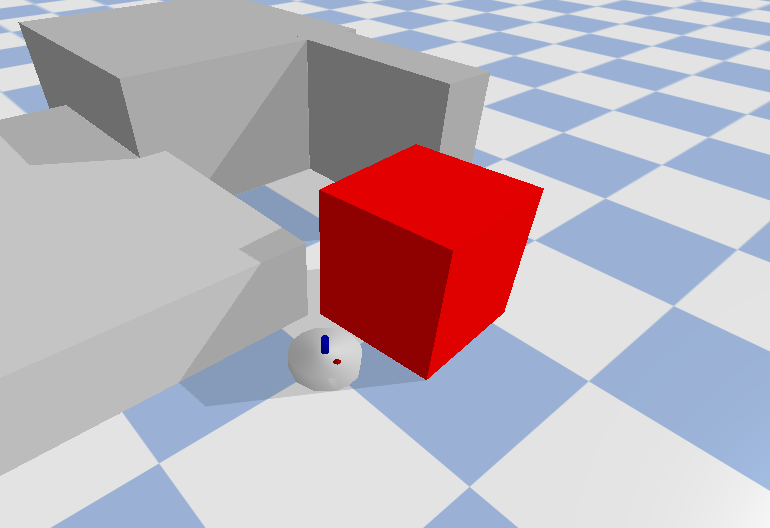
\includegraphics[width=0.45\textwidth]{figures/proposed_method/connecting_nodes/blocking_obj/robot_1}}\quad
  \subfloat{ 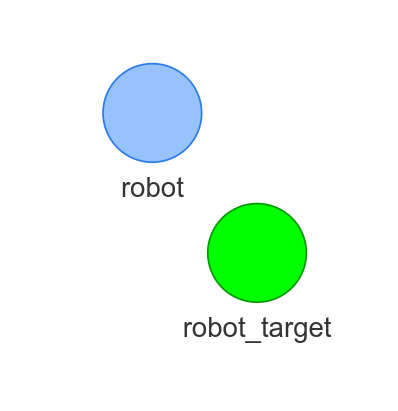
\includegraphics[width=0.35\textwidth]{figures/proposed_method/connecting_nodes/blocking_obj/blocking_obj_0}}
\end{figure}
  \end{center}
\end{frame}


\begin{frame}[fragile]{Proposed Method: H-Algorithm}
  \begin{center}
\begin{figure}
  \centering
  \subfloat{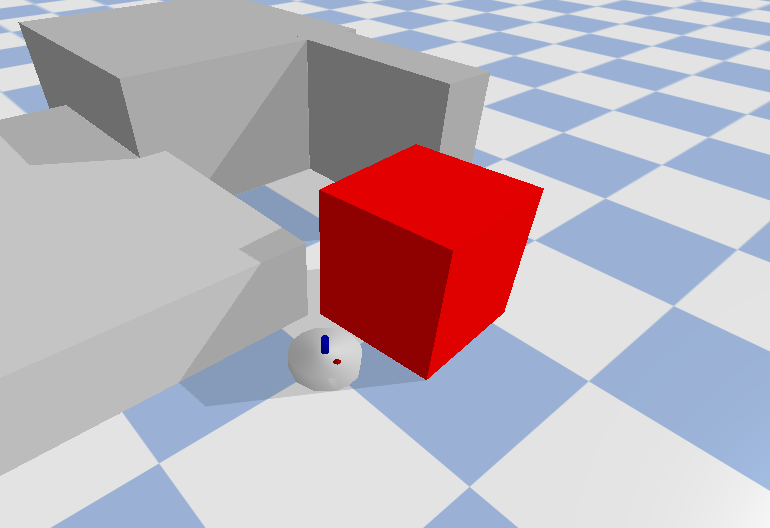
\includegraphics[width=0.45\textwidth]{figures/proposed_method/connecting_nodes/blocking_obj/robot_1}}\quad
  \subfloat{ 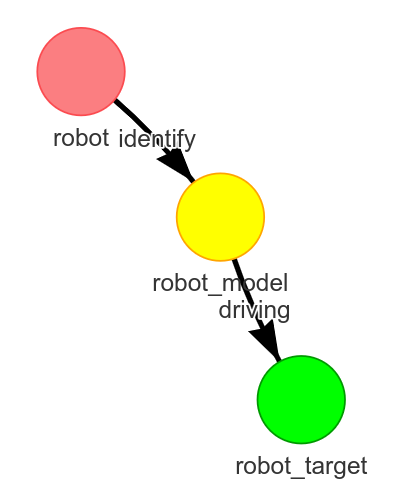
\includegraphics[width=0.32\textwidth]{figures/proposed_method/connecting_nodes/blocking_obj/blocking_obj_2}}
\end{figure}
  \end{center}
\end{frame}

\begin{frame}[fragile]{Proposed Method: H-Algorithm}
  \begin{center}
\begin{figure}
  \centering
  \subfloat{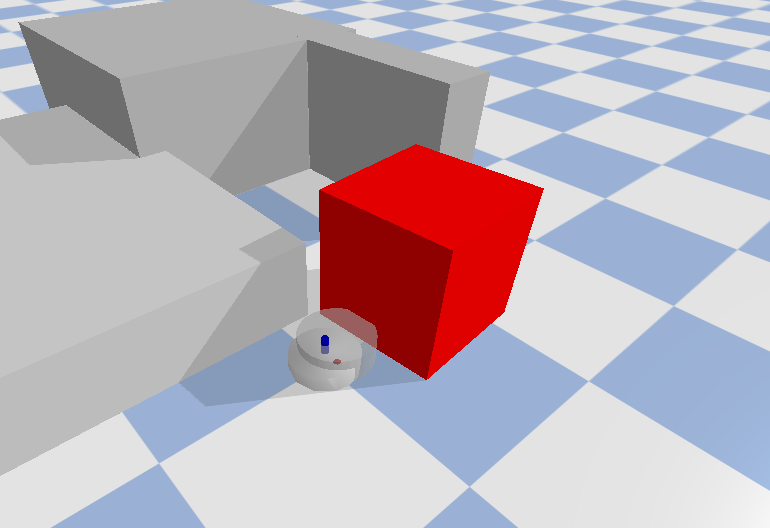
\includegraphics[width=0.45\textwidth]{figures/proposed_method/connecting_nodes/blocking_obj/robot_0}}\quad
  \subfloat{ 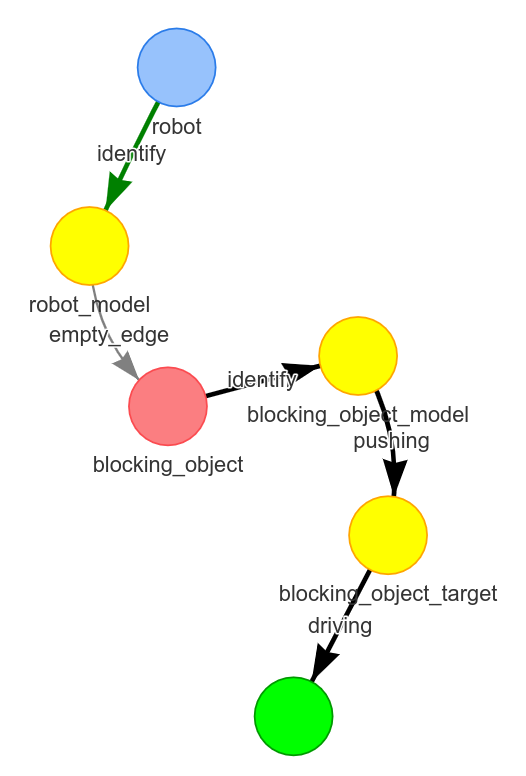
\includegraphics[width=0.35\textwidth]{figures/proposed_method/connecting_nodes/blocking_obj/blocking_obj_3}}
\end{figure}
  \end{center}
\end{frame}

\begin{frame}[fragile]{Proposed Method: H-Algorithm}
  \begin{center}
\begin{figure}
  \centering
  \subfloat{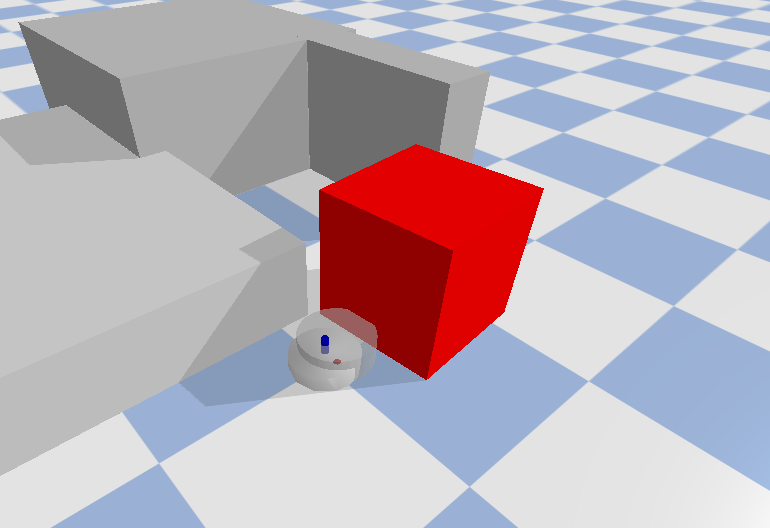
\includegraphics[width=0.45\textwidth]{figures/proposed_method/connecting_nodes/blocking_obj/robot_0}}\quad
  \subfloat{ 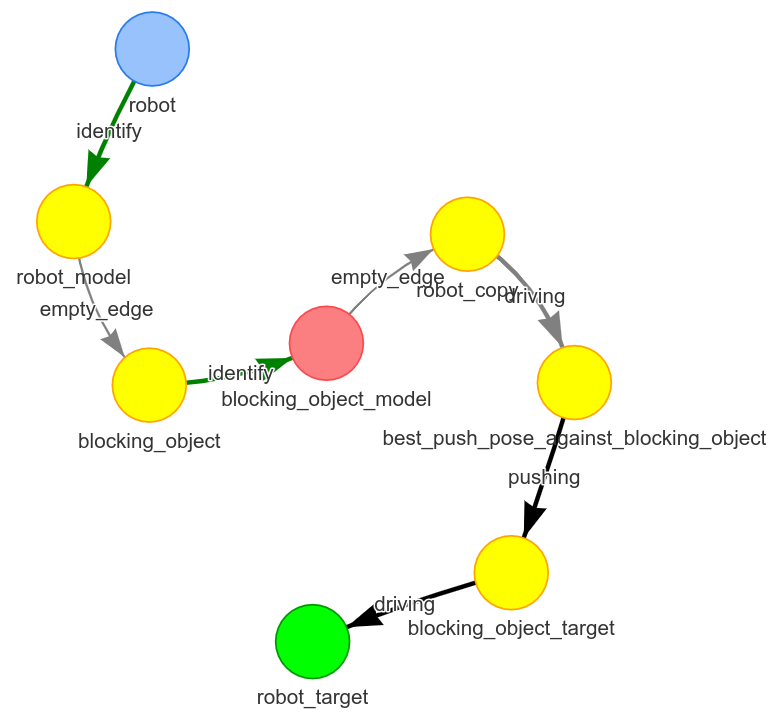
\includegraphics[width=0.45\textwidth]{figures/proposed_method/connecting_nodes/blocking_obj/blocking_obj_4}}
\end{figure}
  \end{center}
\end{frame}

\begin{frame}[fragile]{Proposed Method: H-Algorithm}
  \begin{center}
\begin{figure}
  \centering
  \subfloat{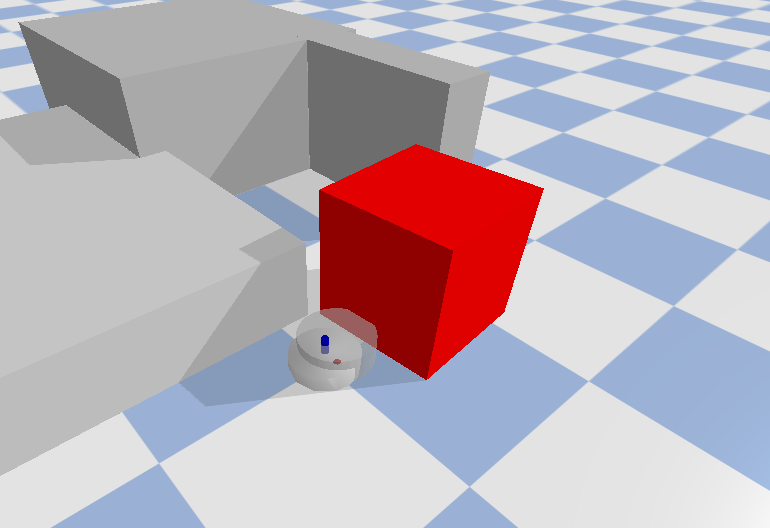
\includegraphics[width=0.45\textwidth]{figures/proposed_method/connecting_nodes/blocking_obj/robot_0}}\quad
  \subfloat{ 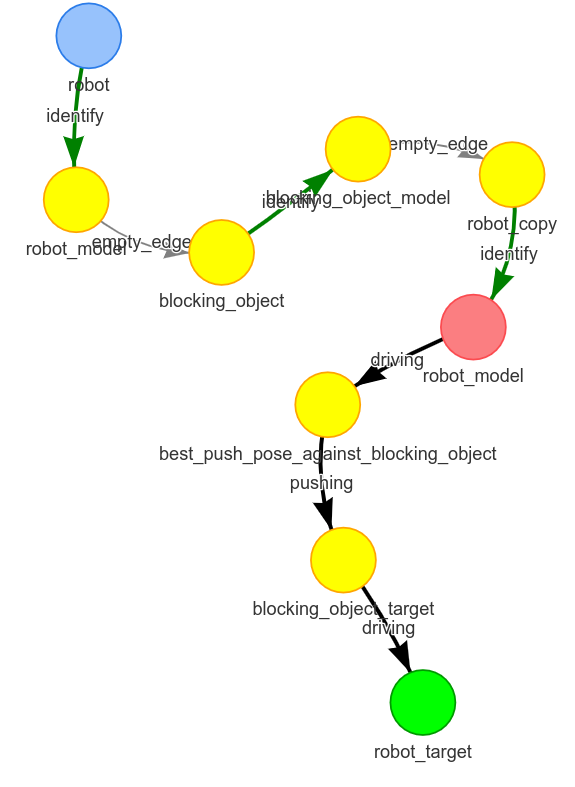
\includegraphics[width=0.30\textwidth]{figures/proposed_method/connecting_nodes/blocking_obj/blocking_obj_5}}
\end{figure}
  \end{center}
\end{frame}

\begin{frame}[fragile]{Proposed Method: H-Algorithm}
  \begin{center}
\begin{figure}
  \centering
  \subfloat{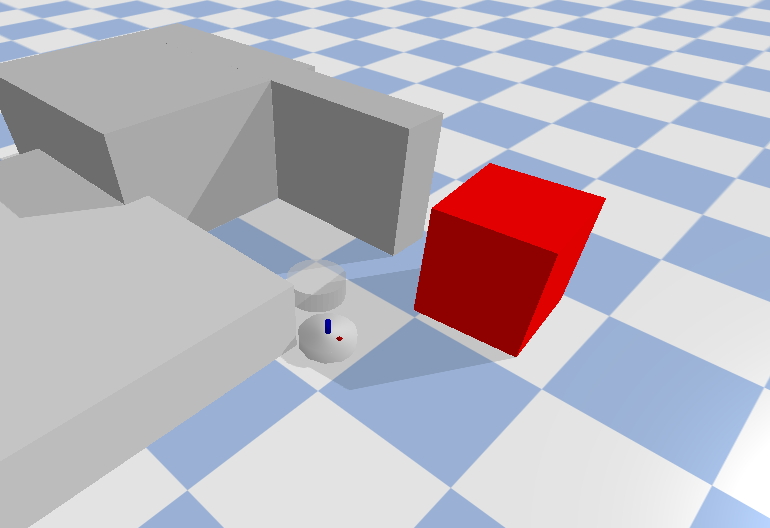
\includegraphics[width=0.45\textwidth]{figures/proposed_method/connecting_nodes/blocking_obj/robot_3}\vspace{2cm}}\quad
  \subfloat{ 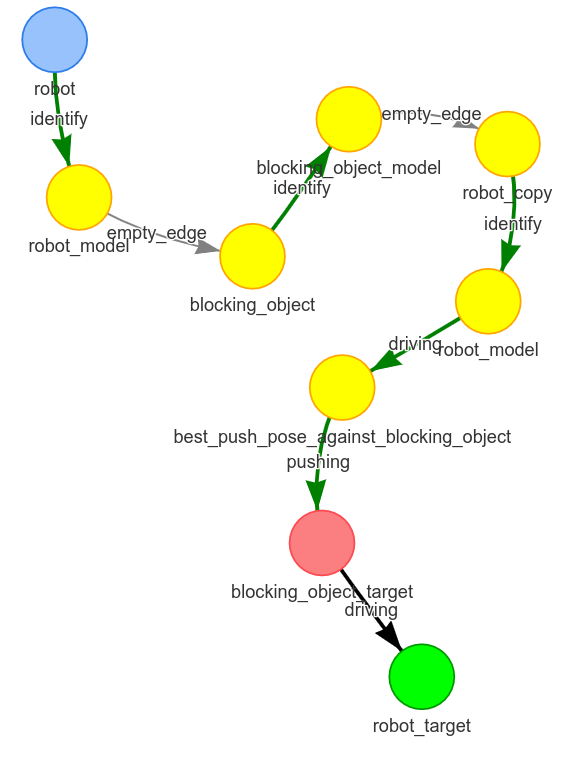
\includegraphics[width=0.35\textwidth]{figures/proposed_method/connecting_nodes/blocking_obj/blocking_obj_6}}
\end{figure}
  \end{center}
\end{frame}

% ROBOT PUSHING
\begin{frame}[fragile]{Proposed Method: H-Algorithm}
  \todo{robot pushing si missing here}
  \begin{center}
\begin{figure}
  \centering
  \subfloat{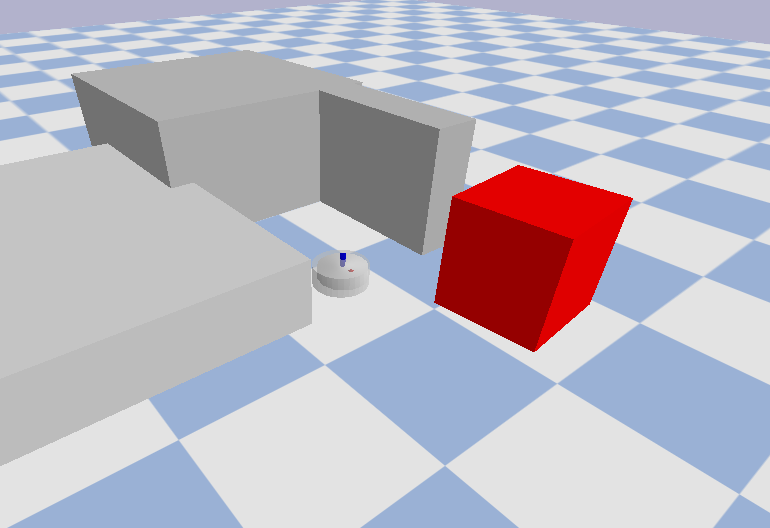
\includegraphics[width=0.45\textwidth]{figures/proposed_method/connecting_nodes/blocking_obj/robot_4}\vspace{2cm}}\quad
  \subfloat{ 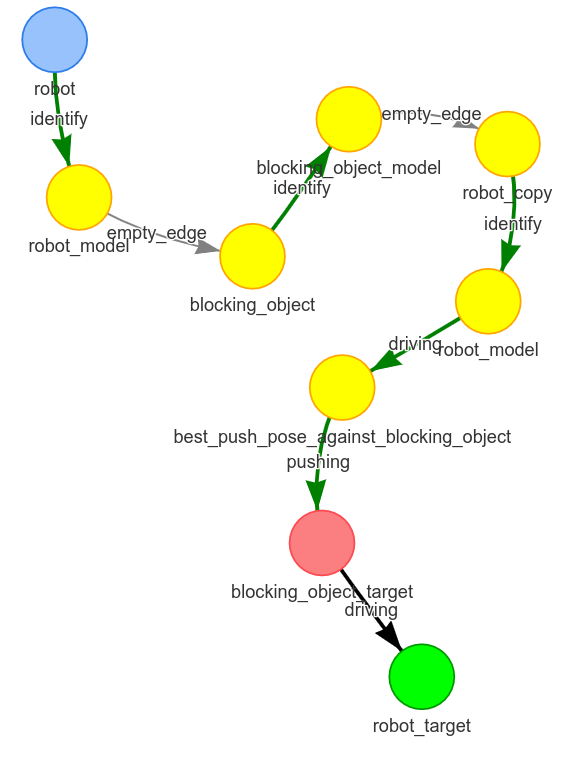
\includegraphics[width=0.35\textwidth]{figures/proposed_method/connecting_nodes/blocking_obj/blocking_obj_6}}
\end{figure}
  \end{center}
\end{frame}

\begin{frame}[fragile]{Proposed Method: H-Algorithm}
  \begin{center}
  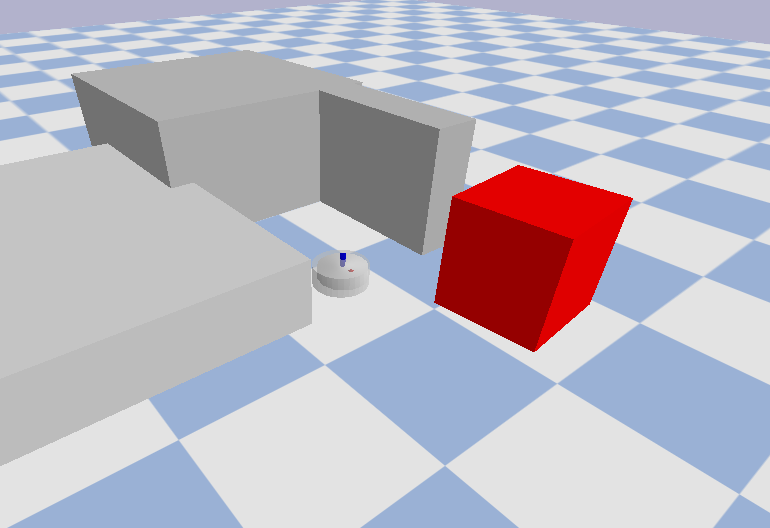
\includegraphics[width=0.45\textwidth]{figures/proposed_method/connecting_nodes/blocking_obj/robot_4}
  \end{center}
\end{frame}


\begin{frame}[fragile]{Proposed Method: H-Algorithm}
  \vspace{-0.5cm}
  \begin{center}
    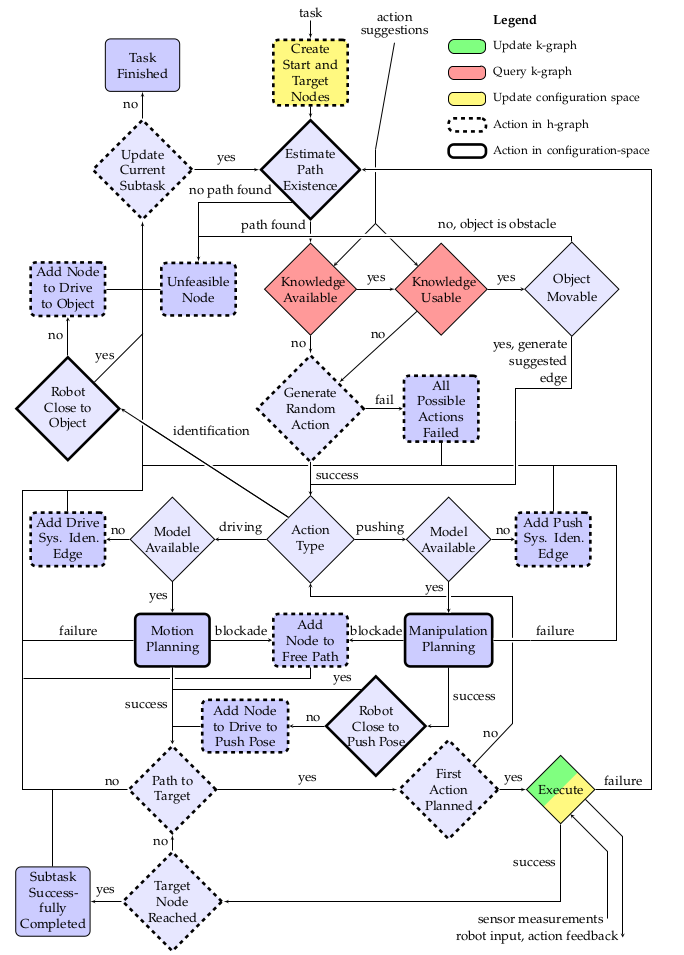
\includegraphics[height=0.9\textheight]{figures/proposed_method/tikz_flowchart_halgorithm}
  \end{center}
\end{frame}

\begin{frame}[fragile]{Proposed Method: H-Algorithm} 
  \vspace{-0.5cm}
  \begin{center}
    \hbox{\hspace{1.5cm} 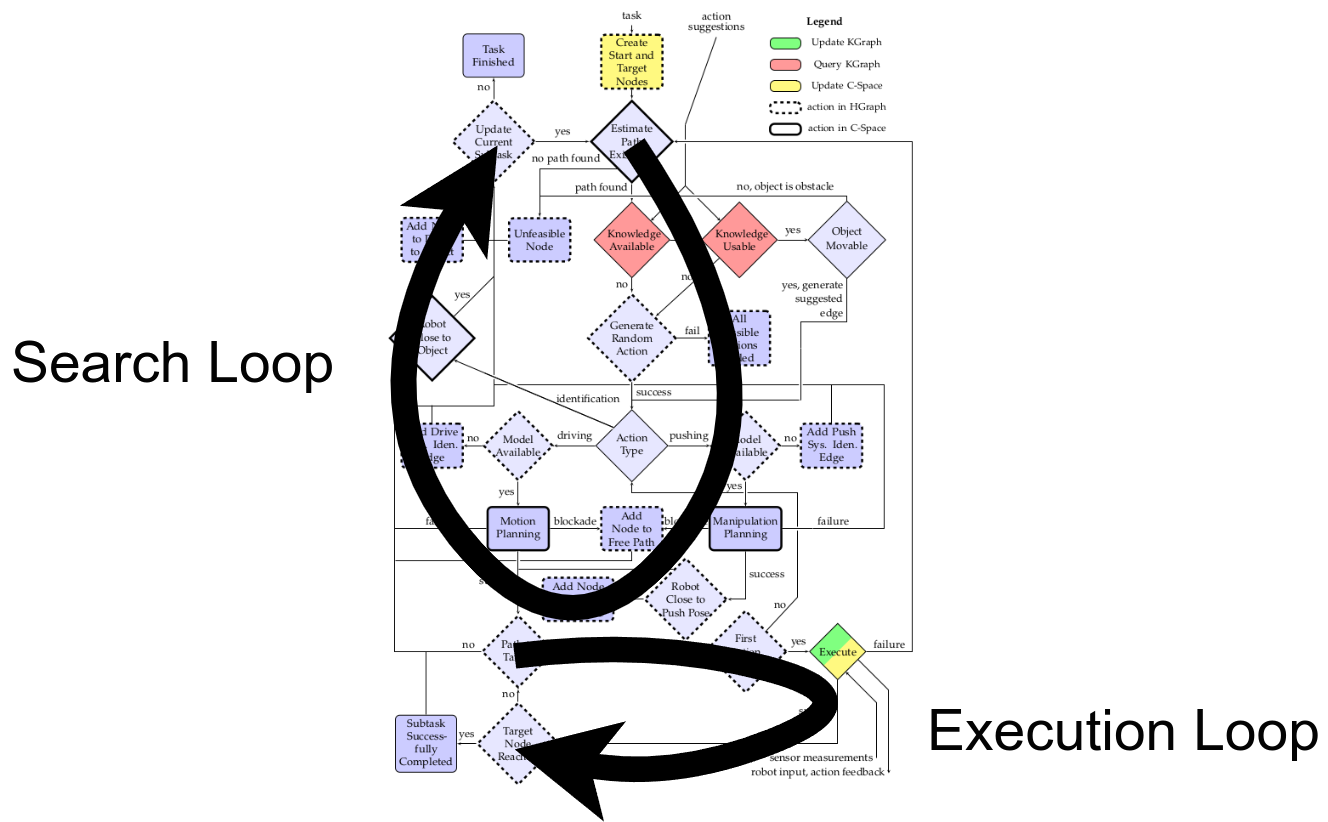
\includegraphics[height=0.9\textheight]{figures/proposed_method/two_loops_identified}}
  \end{center}
\end{frame}

\begin{frame}[fragile]{Proposed Method: H-Algorithm} 
  \todo{explain that the h-algorithm:
  - searches the target node
- connects with edges to the starting node with a backward search
- propagates the states of hypothesis
- executs the hypotheis}
\end{frame}

% \begin{frame}[fragile]{Proposed Method: H-Algorithm} 
%   \begin{center}
%     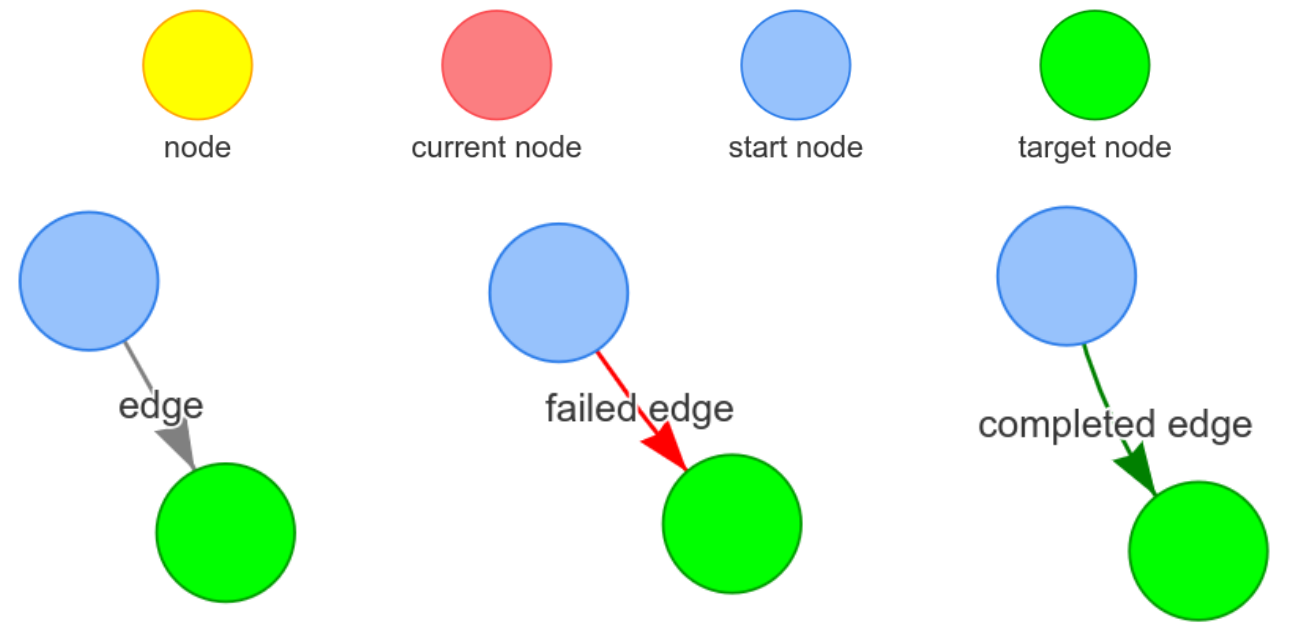
\includegraphics[width=1.0\textwidth]{figures/proposed_method/hgraph_legend}
%   \end{center}
% \end{frame}


% \begin{frame}[fragile]{Proposed Method: H-Algorithm} 
% \begin{center}
%   \todo{make a push a box image}
% \end{center}
% \end{frame}

% \begin{frame}[fragile]{Proposed Method: H-Algorithm} 
% \begin{center}
%   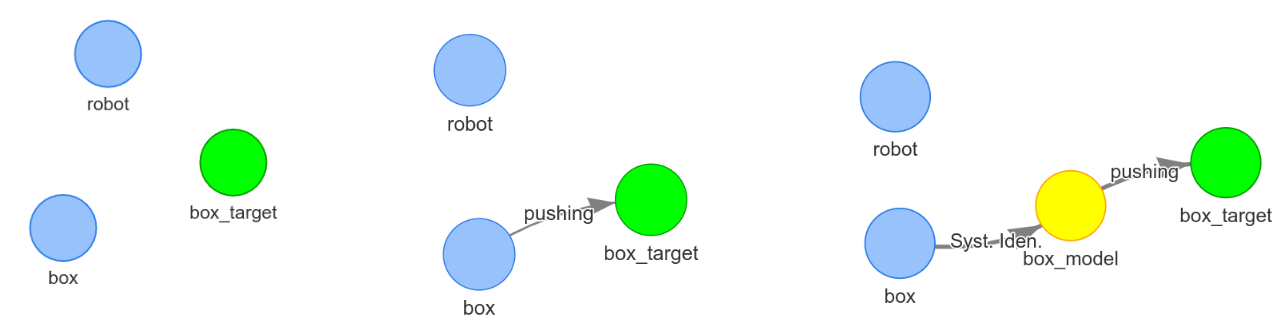
\includegraphics[width=1.0\textwidth]{figures/proposed_method/hgraph_example1}\pause

%   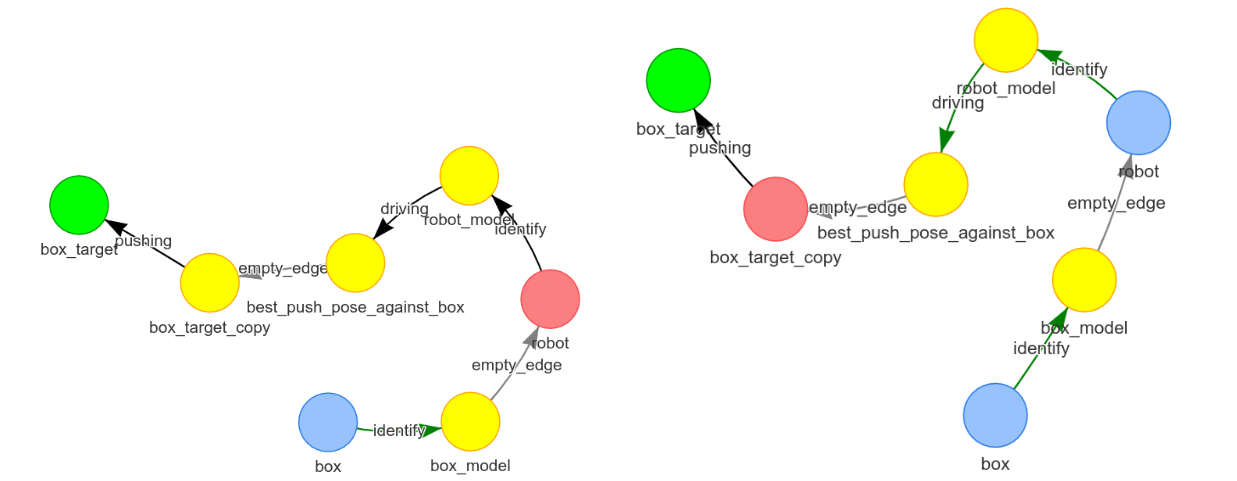
\includegraphics[width=1.0\textwidth]{figures/proposed_method/hgraph_example2}
% \end{center}
% \end{frame}

% \begin{frame}[fragile]{Proposed Method: H-Algorithm} 
%   \begin{center}
%     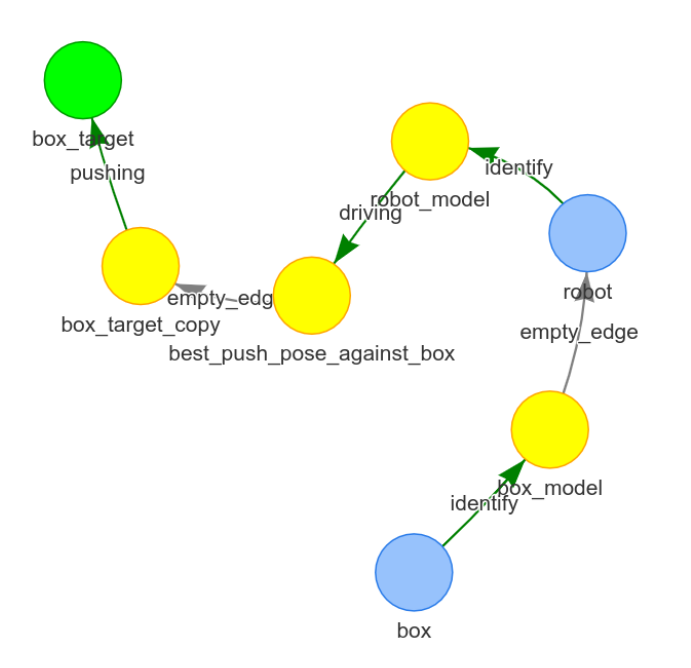
\includegraphics[width=0.5\textwidth]{figures/proposed_method/hgraph_example3}
%   \end{center}
% \end{frame}

\begin{frame}[fragile]{Proposed Method: H-Algorithm} 
\begin{block}{Halgorithm behaviour}
    \begin{itemize}
      \item Fault detection $\rightarrow$ fail edge
      \item Blocking obstacle $\rightarrow$ free path 
      \item Stop regeneration of failed edges $\rightarrow$ blocklist
    \end{itemize}
  \end{block}
\end{frame}
